\chapter{Compton camera data format}

\section{Introduction}

This document aims to formalize and fix the Compton camera data format. The structure of the data sent by each detector section (scatterer, absorber and beam hodoscope) to the acquisition card is detailed, as well as the structure of the events sent to the acquisition PC.


\section{General features}


\subsection{Common information}

The detector Front End cards are connected to the \charmu-TCA via optical links, with a speed of 3.0 Gbit/s. The transfer frequency is 150 MHz.\newline
All the Front End card TDCs share the same synchronized clock, at a 40 MHz frequency, which is sent to the cards through an external link.\newline
Every data packet sent to the \charmu-TCA by the Front End cards starts with the following information:
\begin{itemize}
	\item N$^{\circ}$ Front End (8 bits);
	\item N$^{\circ}$ Trigger (24 bits);
	\item N$^{\circ}$ Mode (8 bits);
	\item N$^{\circ}$ of element in the packet (8 bits).
\end{itemize}

\subsubsection{Front End number\newline}

The Front End number is the identification code of each Front End card. A mechanical switch on the card defines the ID which is sent in the data packet header.
\newline
In \tablename~\ref{table::FE_numbers} the Front End number IDs are listed with the corresponding cards.

\definecolor{Gray}{gray}{0.9}
\begin{table} [!htbp]
\centering
\caption{Front End number associated to each Front End card.}
\label{table::FE_numbers}
\begin{tabular}{cc}
\hline
\rowcolor{Gray}
\textbf{FE number} & \textbf{FE card} \\
\hline
\hline
0			&	All detectors \\
\hline
1			 &     Silicon 1\\
2			&	Silicon 2	\\
3        		&	Silicon 3	\\
4			&	Silicon 4	\\
5			 &     Silicon 5\\
6			&	Silicon 6	\\
7        		&	Silicon 7	\\
8			&	Silicon 8	\\
9        		&	Silicon 9	\\
10			&	Silicon 10\\
\hline
11			&	ASM 1\\
12			&	ASM 2\\
13			&	ASM 3\\
14			&	ASM 4\\
15			&	ASM 5\\
16			&	ASM 6\\
17			&	ASM 7\\
18			&	ASM 8\\
19			&	ASM 9\\
20			&	ASM 10\\
21			&	ASM 11\\
22			&	ASM 12\\
23			&	ASM 13\\
24			&	ASM 14\\
25			&	ASM 15\\
26			&	ASM 16\\
\hline
27			 &     Hodoscope 1\\
28			&	Hodoscope 2	\\
29        		&	Hodoscope 3	\\
30			&	Hodoscope 4	\\
31			 &     Hodoscope 5\\
32			&	Hodoscope 6	\\
33        		&	Hodoscope 7	\\
34			&	Hodoscope 8	\\
\hline
99 			&  \charmu-TCA\\
\hline
\end{tabular}
\end{table}


\subsubsection{Pre-trigger and trigger\newline}

The trigger number identifies each event, where an event is generated every time a coincidence is detected between a BGO block and a silicon layer. Once an interaction is detected in a BGO block, the associated ASM card generates a pre-trigger signal which is sent to the THOR card. This intermediate card shares the pre-trigger signal with the silicon FE cards; if an interaction with a compatible time stamp is found in one of the silicon layer, a trigger signal is generated and sent to all the silicon FE card, as well as to the ASM and hodoscope cards via the THOR card. The trigger signal validates the event, and each FE card sends the collected data to the \charmu-TCA system. The trigger number allows for a complete event reconstruction by the event builder on the acquisition PC. In \figurename~\ref{fig::triggerGeneration} the trigger generation process is sketched.\newline
To be noticed that each FE cards sends the collected data independently from the others.\newline


\underline{Trigger and pre-trigger encoding}\newline

Pre-trigger and trigger signals are used by all the detectors to select the collected data to be sent to the acquisition system. The data selection and transfer must be as fast as possible in order to minimize the trigger latency and camera dead time. In order to reduce the transmission time, pre-trigger and trigger signals have been encoded on 24 bits.\newline
This same trigger number is sent at the beginning of each data packet and is used by the event builder to associate the interactions collected by the three detector sections. With a 24-bit encoding, the trigger number is reset every 1 ns $\times \mathrm{2^{24}} =$ 16,78 ms. This time window is short for the event builder, so that for the physical data it is extended to 32 bits for all the FE cards in order to have a reset every 1 ns $\times \mathrm{2^{32}} =$ 4,2 s, which is enough for the reconstruction of the events.

\newpage
\begin{landscape}
\begin{figure} [!h]
\caption{Trigger generation and sharing with the three detector sections.}
 \subfloat[Pre-trigger generation in the THOR card.]{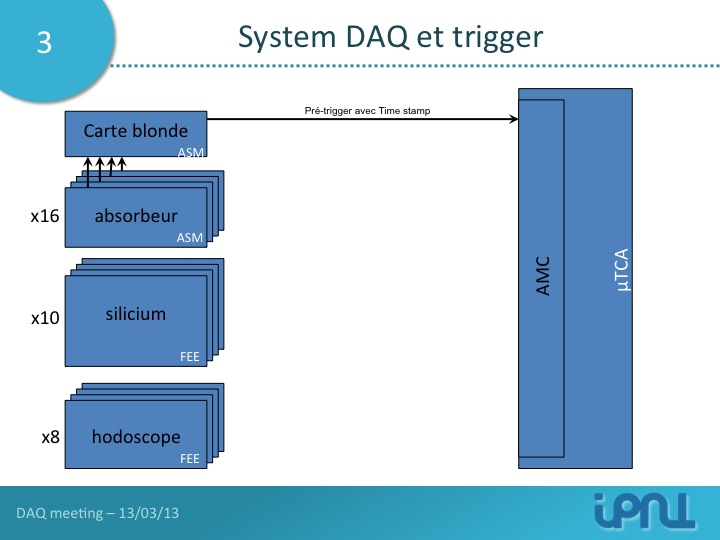
\includegraphics[width=0.5\textwidth]{03_GraphicFiles/appendixA_dataFormat/DAQ_update_13-03-15_Diapositive03.jpg}}
 \subfloat[Pre-trigger sent to the 10 silicon FE cards.]{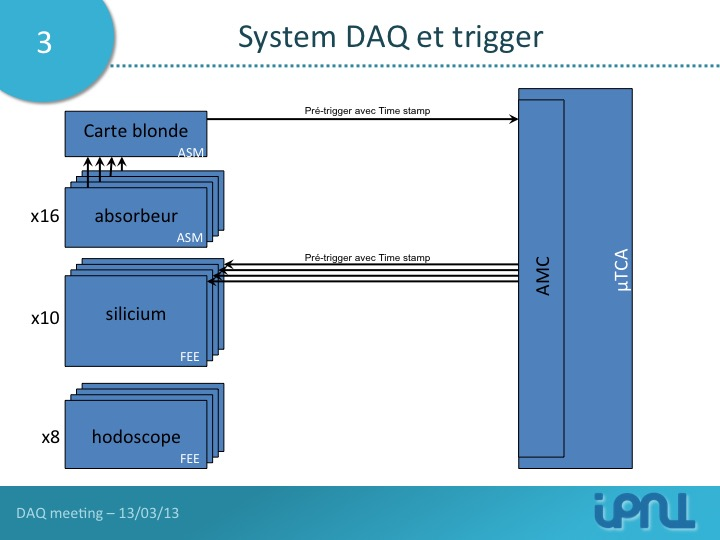
\includegraphics[width=0.5\textwidth]{03_GraphicFiles/appendixA_dataFormat/DAQ_update_13-03-15_Diapositive04.jpg}}\\
 \subfloat[A single silicon FE card generates the trigger.]{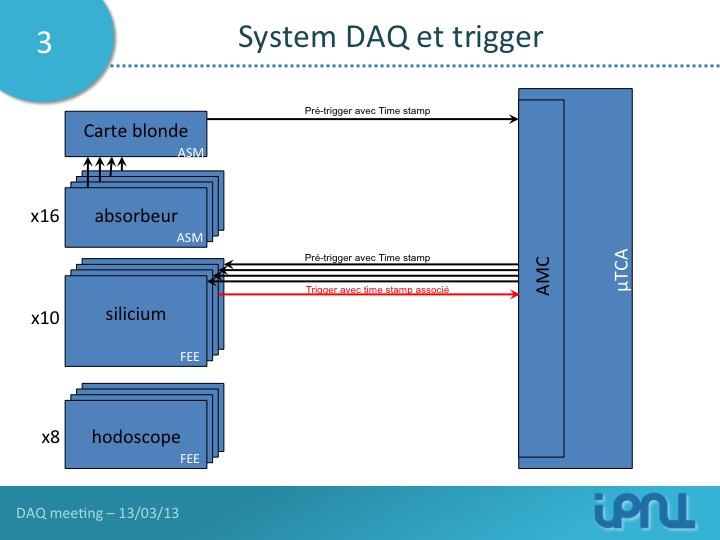
\includegraphics[width=0.5\textwidth]{03_GraphicFiles/appendixA_dataFormat/DAQ_update_13-03-15_Diapositive05.jpg}}
 \subfloat[Trigger signal is distributed to all the detectors.]{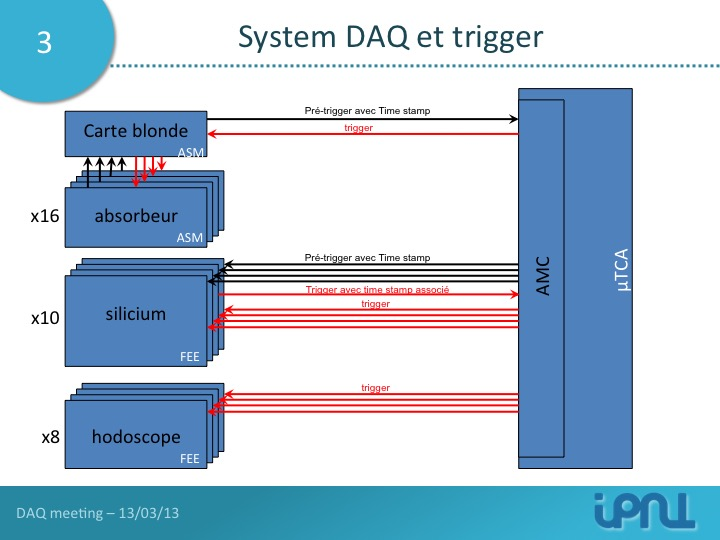
\includegraphics[width=0.5\textwidth]{03_GraphicFiles/appendixA_dataFormat/DAQ_update_13-03-15_Diapositive06.jpg}}\\
 \subfloat[The detectors send the collected data to the \charmu-TCA. ]{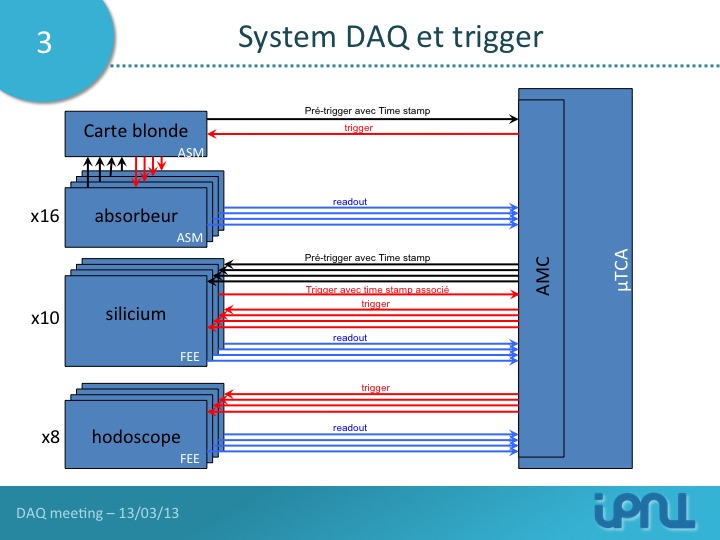
\includegraphics[width=0.5\textwidth]{03_GraphicFiles/appendixA_dataFormat/DAQ_update_13-03-15_Diapositive07.jpg}}
  \label{fig::triggerGeneration}
\end{figure}
\end{landscape}


\subsubsection{Mode number\newline}

The Compton camera detector components can work in different mode, according to the application requirements. At least two working modes are possible for every detector section: an \enquote{optimal} mode, corresponding to the final camera configuration; a \enquote{test} mode, allowing for the collection of more raw information. Every operating mode presents a peculiar data format, so that the data packets size is not fixed. In order to fix the acquisition tuning, the mode number is defined before its beginning.\newline
The operating mode are identified as following: \newline
\begin{itemize}
	\item N$^{\circ}$ Mode = 1 : $1^{\mathrm{st}}$ mode for silicon
	\item N$^{\circ}$ Mode = 2 : $2^{\mathrm{nd}}$ mode for silicon
	\item N$^{\circ}$ Mode = 3 : $3^{\mathrm{rd}}$ mode for silicon
	\item N$^{\circ}$ Mode = 4 : $4^{\mathrm{th}}$ mode for silicon
	\item N$^{\circ}$ Mode = 5 : $1^{\mathrm{st}}$ mode for BGO
	\item N$^{\circ}$ Mode = 6 : $2^{\mathrm{nd}}$ mode for BGO
	\item N$^{\circ}$ Mode = 7 : $1^{\mathrm{st}}$ mode for hodoscope
	\item N$^{\circ}$ Mode = 8 : $2^{\mathrm{nd}}$ mode for hodoscope.\newline
\end{itemize}

%La description des différentes possibilités est détaillée par les figures 2, 3 et 4.


\section{Physical data format}

%\subsection{Format spécifique pré-trigger et trigger}

%Le format pour ces deux informations est simplement constitué d'une information: le time stamp.

\subsection{Scatterer detector data format}

Four different data formats, corresponding to four working modes, have been defined for the silicon scatterer operation (figure 2). For mode 1 and 2, the collected total charge is directly evaluated on the FE card via the slow shaper output and one ASIC, while for mode 3 and 4 the ASIC pre-amplifier output directly sends a sampling of the raw signal.  In this last case, the number of samples can be tuned and each sample corresponds to 10 ns.The complete sampling is stored in a dedicated buffer (see table 9).\newline\newline
\underline{Modes 1 and 3}\newline
In mode 1 and 3, for each detector strip involved in the interaction, the strip ID, total collected charge and time are stored. The interaction position will be calculated via a center of gravity algorithm at the analysis stage. The raw information about the number of involved strips is useful for the evaluation of the signal dispersion in the detector.\newline
\underline{Modes 2 and 4}\newline
In mode 2 and 4, the interaction is calculated on the FE card and the number of involved strip is then not stored.

	\begin{figure} [hbtp]
	\centering
	\caption{Silicon scatterer data format.}
	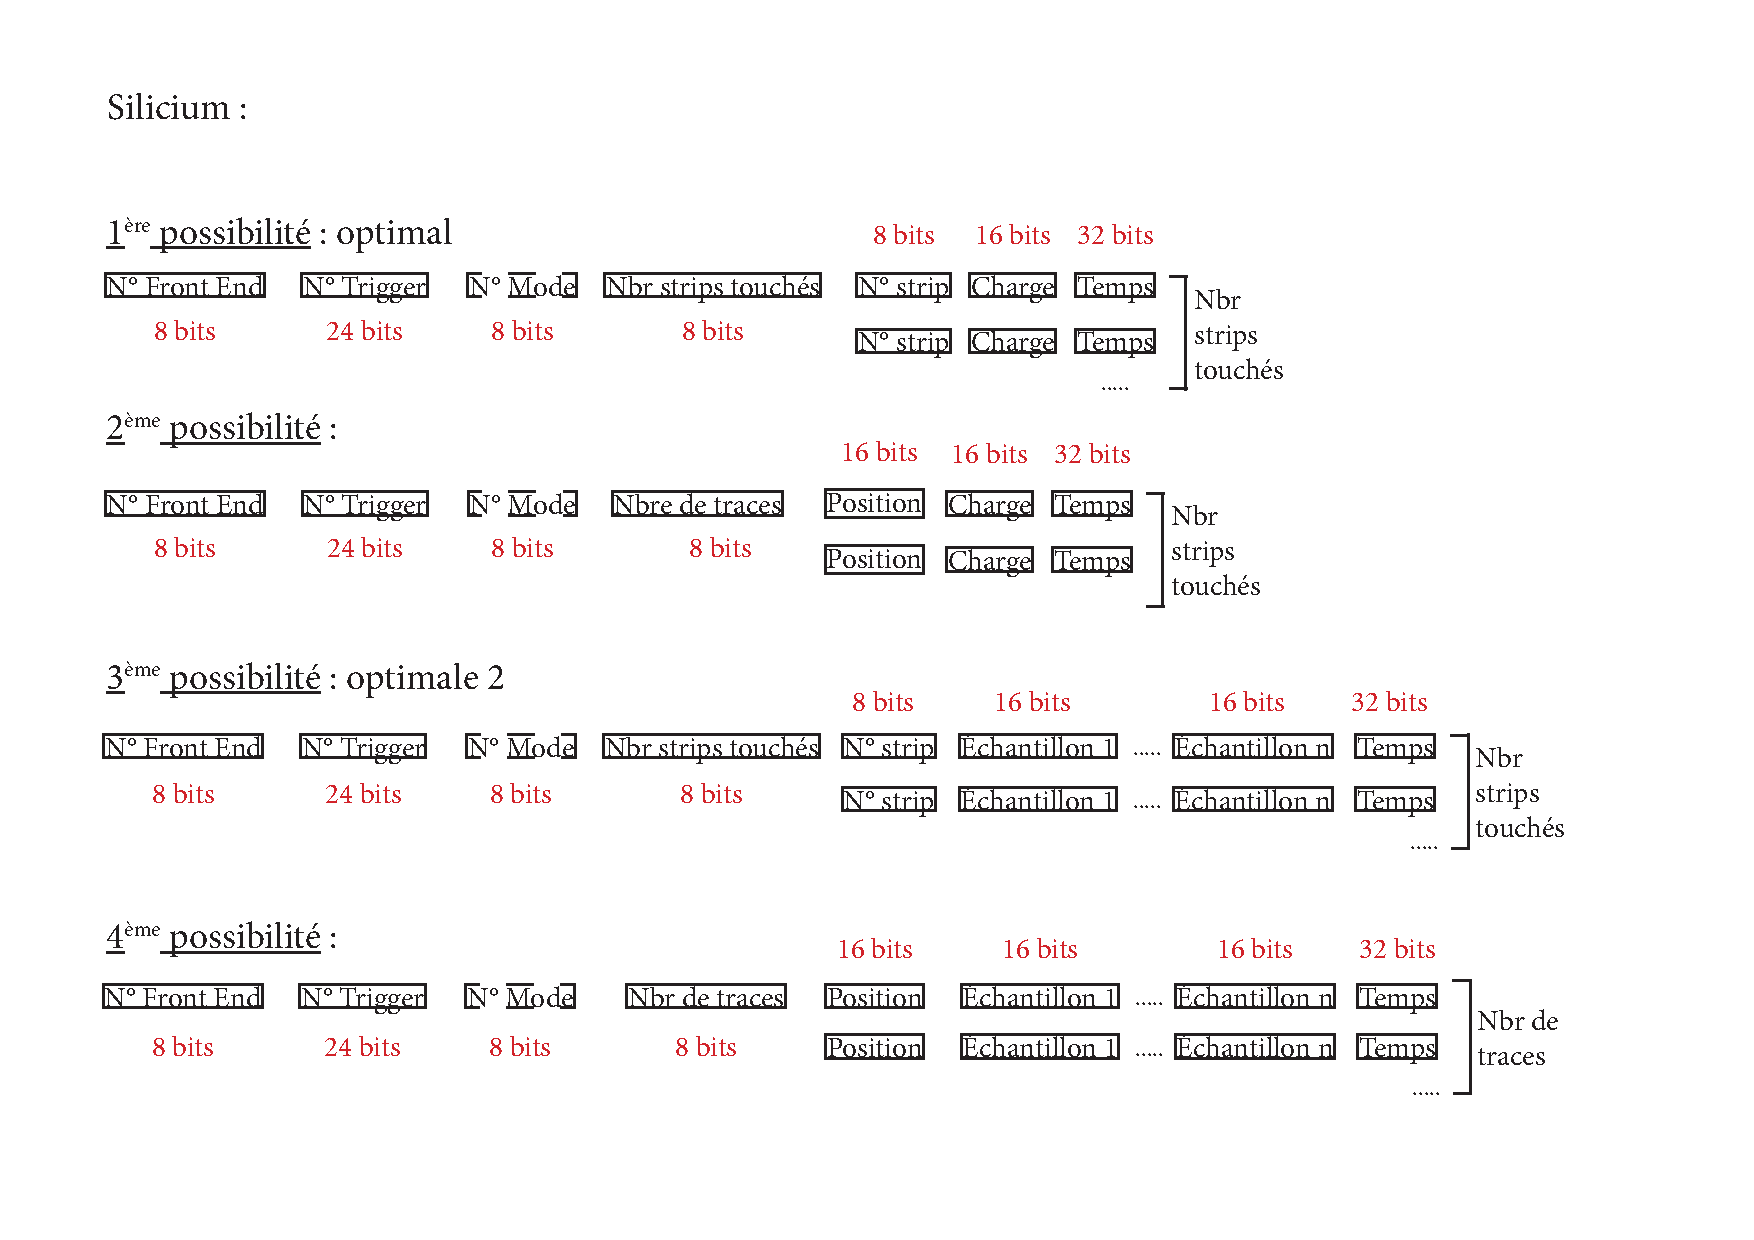
\includegraphics[width=1.3\textwidth]{03_GraphicFiles/appendixA_dataFormat/2015_05_14_Format_datas_acquisition_Si.pdf}
	\end{figure}

\clearpage
\newpage
\subsection{Absorber detector data format}
The BGO block readout is performed via the ASM cards. Each card is equipped with 24 input ports (signal PM), corresponding to 6 BGO blocks. Two possible working modes have been defined for the BGO absorber: the collected total charge and time are evaluated on the card, or the PM raw signals are sampled and the sampling is sent to the acquisition (figure 3). Charge and time are then calculated at the analysis stage. This second operating mode can be useful in the test phase but it determines a low acquisition rate, so that it can be used only at low beam intensity.\newline
The complete sampling is stored in a dedicated buffer (see table 9).

  	\begin{figure} [hbtp]
	\centering
	\caption{BGO absorber data format.}
	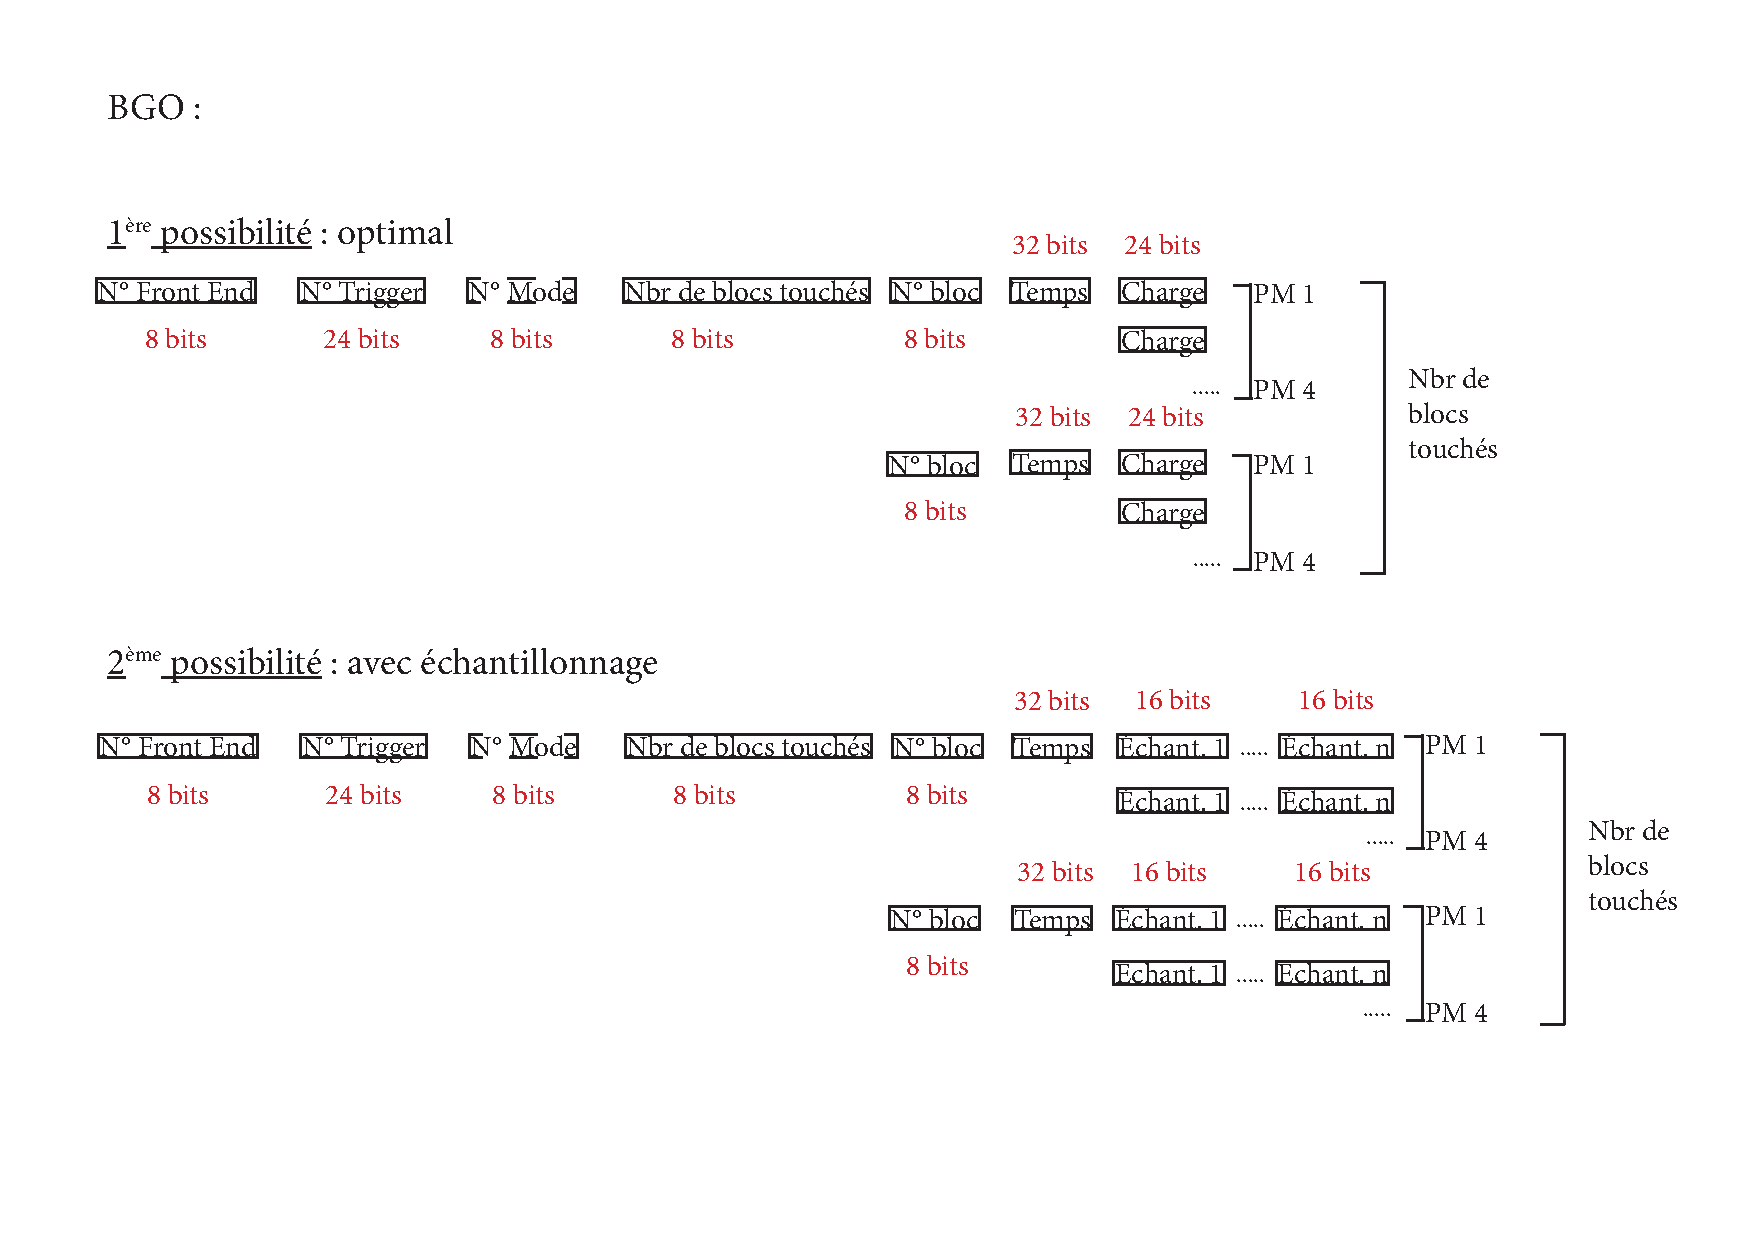
\includegraphics[width=1.2\textwidth]{03_GraphicFiles/appendixA_dataFormat/2015_05_14_Format_datas_acquisition_BGO.pdf}
	\end{figure}



\clearpage
\subsection{Beam hodoscope data format}
The beam tagging hodoscope is composed of two perpendicular planes of 128 scintillating fibers each. Each fiber is read-out on the two sides, for a total of  512 read-out channels. The output signals are send via optical fibers to 8 64-channel PM H8500 by Hamamatsu. 8 FE cards have been developed for the signal collection, one per PM, and are equipped with two custom ASICs (32 channels each) and one FPGA.\newline
Concerning the \enquote{optimal} mode (1$^{\mathrm{st}}$ operating mode for the hodoscope), the only collected information are the ID of the involved fibers and the interaction time. The ASICs allow for a minimum time resolution of 10 ns; this means that if two particles interacts in the hodoscope within a 10 ns window, they will be considered as part of a single event.\newline
In test mode, the total collected charge can be calculated. This feature is useful to evaluate the detector aging effect due to radiation exposure. The charge measurement is anyway limited to a single channel per ASIC, so to two channels per PM. The ASIC channel able to measure the charge is identified as "N$^{\circ}$ Fiber charge 1" and "N$^{\circ}$ Fiber charge 2".

	\begin{figure} [!hbtp]
	\centering
	\caption{Hodoscope data format.}
	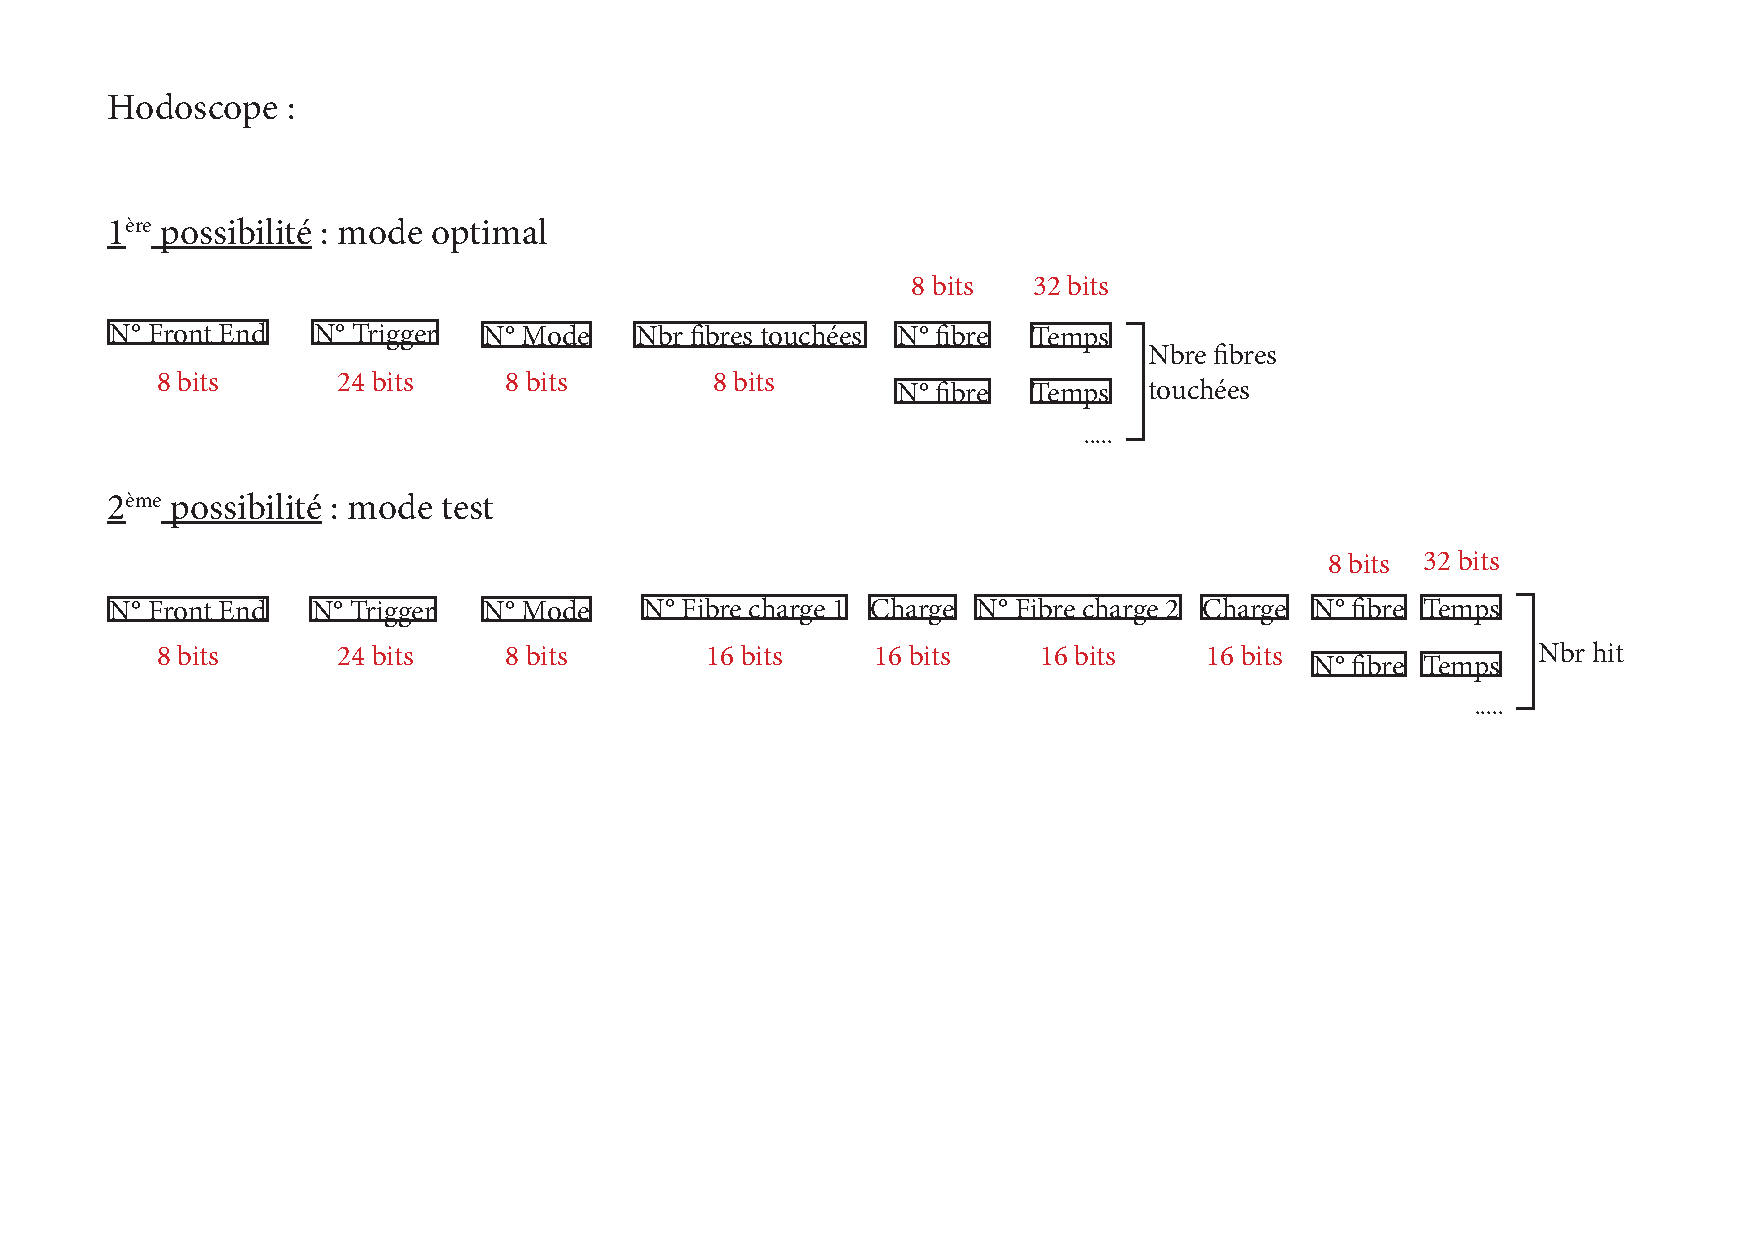
\includegraphics[width=1\textwidth]{03_GraphicFiles/appendixA_dataFormat/2015_01_26_Format_datas_acquisition_hodoscope_update.pdf}
	\end{figure}

%%%%%%%%%%%%%%%%%%%%%%%%%%%%%%%%%%%%%%%%%%%%%%%%%%%%%%%%%%%%%%%%%%%%%%%%
%%%%%%%%%%%%%%%%%%%%%%%%%%%%%%%%%%%%%%%%%%%%%%%%%%%%%%%%%%%%%%%%%%%%%%%%
%%%%%%%%%%%%%%%%%%%%%%%%%%%%%%%%%%%%%%%%%%%%%%%%%%%%%%%%%%%%%%%%%%%%%%%%


\clearpage
\newpage
\section{Slow control, trigger and monitoring data format}

by X. Chen and Y. Zoccarato.

\subsection{Communication architecture}

The Endpoint architecture is composed of three parts:
\begin{itemize}
	\item application
	\item mac (or transport part)/processor packet
	\item physics
\end{itemize}

	\begin{figure} [!hbtp]
	\centering
	\caption{Architecture of communication between DAQ cards and \charmu-TCA.}
	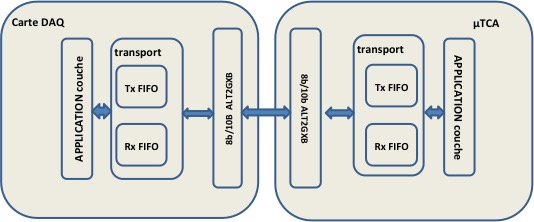
\includegraphics[width=1\textwidth]{03_GraphicFiles/appendixA_dataFormat/architecture_EndPont_update.jpg}
	\end{figure}

\subsection{Transport protocol and processor packets}

\subsubsection{Definitions\newline}
	It is worth to define some useful terms for the following part of the document:

	\begin{itemize}
		\item octet : 8 bits
		\item mot : 16 bits
		\item K : control octet
		\item D : data octet
		\item cargo : data group
		\item terminaison : packet end
		\item CRC : cyclic redundancy code \newline
	\end{itemize}

The CRC allows one to detect the transmission errors and the data transfer issues. A specific algorithm must be used, as CRC-16 : X16 + X15 + X2 + 1. In the present protocol, a \enquote{parity patter of 16 bits} have been used.

The trasport part ensures a proper packets exchange between two terminals via the data shaping. The data come from the application part and are then sent to the physics part.\newline
%\textbf{L'encapsulation choisie est 8 bits/10 bits.}\newline

\subsubsection{Data encoding\newline}
For the transport part, the data structure is created via the addition of a packet header, corresponding to a parity bit, of a 16 bit parity pattern and a bit for the end of the packet.
The data to be sent are encoded with a logic 8bits/10bits. This encoding structure allows for the extraction of the clock from the data flow at the reception time.

\subsubsection{Packets format\newline}

All the data packets have the same structure. A K octet (control) is followed by the cargos to be sent. The end of the packets changes according to the cargos parity.\newline
If the cargo contains an even number of octets, the packet ends with K.28.6.
\begin{table} [!htbp]
  \centering
  \caption{Packet with an even octet number cargo.}
\begin{tabular}{|c|p{4cm}|p{4cm}|p{4cm}|p{4cm}|}
\hline
\bf{Item}  & 		\bf{Packet beginning}		& \bf{Cargo}	& \bf{Packet end}\\
\hline
1			&	One K octet 	& 0 - N D-octets			&		K.28.6	\\
\hline
\end{tabular}
\end{table}

If the cargo contains an odd number of octets, the packet ends without any particul octet.

\begin{table} [!htbp]
  \centering
  \caption{Packet with an odd octet number cargo.}
\begin{tabular}{|c|p{4cm}|p{4cm}|p{4cm}|p{4cm}|}
\hline
\bf{Item}  & 		\bf{Packet beginning}		& \bf{Cargo}	& \bf{Packet end}\\
\hline
1			&	One K octet	&	0 - N D-octets				&	Start of a new packet	\\
\hline
\end{tabular}
\end{table}

\underline{Remark} :
	\begin{itemize}
		\item SYN packet is a special kind of packet starting with K.28.6 and ending with K.28.5. It is only composed of these two octets (16 bits). It allow the receiver to find the beginning and the end of the transmitted octets with the aim to reconstruct the events in parallel. The synchronization speed is 44 Hz (data by Carlos Abellan).
		\item In order to optimize the passing band, the K octet at the beginning of the packet can probably be removed (further study needed).
		\end{itemize}

\newpage


\subsubsection{Possible K octets\newline}

In the following table, all the possible K octets are listed (document by Carlos Abellan).

\begin{table} [!htbp]
  \centering
  \caption{K octets definition.}
\begin{tabular}{|c|p{4cm}|p{4cm}|p{4cm}|p{4cm}|}
\hline
\bf{Item}  			& 		\bf{Name}		& \bf{Control code}	& \bf{Comment}\\
\hline
1				&	K.28.0			&	0x1C			&	Acknowledgement\\
2				&	K.28.1			&	0x3C			&	Ask for writing registers\\
3				&	K.28.2			&	0x5C			&	Ask for reading registers\\
4				&	K.28.3			&	0x7C			&	Special command\\
5				&	K.28.4			&	0x9C			&	Monitoring\\
6				&	K.28.5			&	0xBC		& Default synchronization\\
7				&	K.28.6			&	0xDC		& IDLE (default) and packet end\\
8				&	K.28.	7			&	0xFC		&	Pre-trigger\\
9				&	K.23.7			&	0xF7			&	Trigger \\
10				&	K.27.7			&	0xFB			&	\\
11				&	K.29.7			&	0xFD			&	\\
12				&	K.30.7			&	0xFE			&	Physical data\\
\hline
\end{tabular}
\end{table}

\clearpage
\newpage

\subsection{Trasport part}

\subsubsection{Control packet\newline}

This kind of packet is used to check the link and for the control/command operations.
\begin{itemize}
\item For the link check, two kinds of packets are used: synchronization packet and IDLE packet.
\item For the control/command operation, here are some examples: register configuration,  FPGA dynamical programming, monitoring, etc.\newline
\end{itemize}

\underline{Control octets} :

\begin{table} [!htbp]
  \centering
  \caption{Control octets K definition.}
\begin{tabular}{|c|p{4cm}|p{4cm}|p{4cm}|p{4cm}|}
\hline
\bf{Item}  			& 		\bf{Name}		& \bf{Control code}	& \bf{Comment}\\
\hline
1				&	K.28.0			&	0x1C			& Acknowledgement	\\
2				&	K.28.1			&	0x3C			& Ask for writing registers	\\
3				&	K.28.2			&	0x5C			& Ask for reading registers	\\
4				&	K.28.3			&	0x7C			& Special command	\\
5				&	K.28.4			&	0x9C			& Monitoring	\\
6				&	K.28.5			&	0xBC		& Synchronization	\\
7				&	K.28.6			&	0xDC		& IDLE (default) and end of packet\\
\hline
\end{tabular}
\end{table}


\underline{Acknowledgement packet} (\textit{Front End cards $\rightarrow$ {\charmu-TCA}})\newline

This packet is sent by the FE cards and interpreted as an acknowledgement by the \charmu-TCA. If a part is missing, it is set to zero.
\begin{itemize}
	\item If 0 = validation
	\item If 1 = problem detected
\end{itemize}


\begin{table} [!htbp]
  \centering
  \caption{Definition of the acknowledgement packet.}
\begin{tabular}{|c|p{1.5cm}|p{0.5cm}|p{1cm}|p{1cm}|p{1cm}|p{1cm}|p{1cm}|p{2cm}|p{2cm}|}
\hline
\bf{Word}  			& 		\bf{1$^{st}$ octet}		& \multicolumn{8}{c|}{\bf{2$^{nd}$ octet}} 	\\
\hline
					&						& 7b & 6b& 5b&4b&3b&2b&1b&0b \\
					\cline{3-10}
1				&	K.28.0			&	0	& Pb Front End number & Pb with packet beginning & Pb with packet end & Pb with CRC & Pb with number of received words &  Pb with parity bit of octet 2 & parity bit of the acknowledgement packet	\\
\hline
2				& \multicolumn{9}{c|}{Front End number}\\
\hline
\end{tabular}
\end{table}

\newpage
\subsubsection{Configuration packets\newline}

\underline{Writing register process} (\textit{{\charmu-TCA} $\rightarrow$ Front End cards})\newline

The process starts with a packet sent by the \charmu-TCA asking for the register writing. The receiver (FE card) sends back an acknowledgement packet to finish the process. In the following table the format of this writing register packet is reported.

\begin{table} [!htbp]
  \centering
  \caption{Writing register packet.}
\begin{tabular}{|c|p{4cm}|p{4cm}|p{4cm}|}
\hline
\bf{Word}  			& 	\bf{1$^{st}$ octet}	& \bf{2$^{nd}$ octet} & \bf{Comment} \\
\hline
1				&	K.28.1	& Front End number + 1 parity bit		& N/A  \\
\hline
2				&\multicolumn{2}{p{8cm}|}{2 octets with the number of words to be written}& The length is word-based: max $2^{16}-~1$~=~65535 words\\
\hline
3 			&      \multicolumn{2}{p{8cm}|}{Register address} & Address where the writing process starts\\
\hline
4..N+3        	&      \multicolumn{2}{p{8cm}|}{Data to be written} &0000 0000\\
\hline
N+4				 & \multicolumn{2}{p{8cm}|}{CRC composed of the « xor » of all bits in the same position, from word 2 to word (N+3)}&/\\
\hline
\end{tabular}
\end{table}

\newpage
\underline{Reading register process} (\textit{{\charmu-TCA} $\rightarrow$ Front End cards})\newline

The process starts with a packet sent by the \charmu-TCA asking for the register reading. The receiver (FE card) sends back the \enquote{measure packet} (Table 10) if the command is correct, an acknowledgement packet if it is not.\newline
At the beginning of the slow control, the physical addresses on the FE cards are read at the address 0 (Table 9).\newline
In the following table the format of this reading register packet is reported.



\begin{table} [!htbp]
  \centering
  \caption{Reading register packet.}
\begin{tabular}{|c|p{4cm}|p{4cm}|p{4cm}|}
\hline
\bf{Word}  			& 	\bf{1$^{st}$ octet}	& \bf{2$^{nd}$ octet} & \bf{Comment} \\
\hline
1				&	K.28.2	& Front End number + 1 parity bit &  N/A \\
\hline
2				&\multicolumn{2}{p{8cm}|}{2 octets with the number of words to be read}& The length is word-based: max $2^{16}-~1$~=~65535 words\\
\hline
3 			&      \multicolumn{2}{p{8cm}|}{Address of 1$^{st}$ data to be read} & Address where the reading process starts\\
\hline
4				 & \multicolumn{2}{p{8cm}|}{CRC composed of the « xor » of all bits in the same position, from word 2 to word 3}&/\\
\hline
\end{tabular}
\end{table}

\begin{table} [!htbp]
  \centering
  \caption{Two special registers(\textit{{\charmu-TCA} $\rightarrow$  Front End cards})}
\begin{tabular}{|c|p{6cm}|p{6cm}|}
\hline
\bf{Register address}  			& 	\bf{Details}	& \bf{Comment} \\
\hline
0				&	Front End number		&  No writing rights: register in read-only mode. Hard coded on DAQ card.\\
\hline
1				&    It defines the working modes (Table 1)  & Optimal mode, test mode, collimated camera mode, Compton camera mode, individual detector section test. It is possible to write in the register.  \\
\hline
2				& It defines the detector to test (in single detector test mode)		& Scatterer, absorber, hodoscope.\\
\hline
3 				& BGO number of sampling		& For test mode with the BGO blocks signal sampling.\\
\hline
4				& Silicon number of sampling	& PFor test mode with the silicon layers signal sampling.\\
\hline
\end{tabular}
\end{table}



\newpage


\begin{table} [!htbp]
  \centering
  \caption{Measurement packet. (\textit{Front End cards $\rightarrow$ {\charmu-TCA}})}
\begin{tabular}{|c|p{4cm}|p{4cm}|p{4cm}|}
\hline
\bf{word}  			& 	\bf{1$^{st}$ octet}	& \bf{2$^{nd}$ octet} & \bf{Comment} \\
\hline
1				&	K.28.1	&Front End number + 1 parity bit		&\\
\hline
2				&\multicolumn{2}{p{8cm}|}{2 octets for the number of data words to send}& The length is word-based: max $2^{16}-~1$~=~65535 words\\
\hline
3 			&      \multicolumn{2}{p{8cm}|}{Register address} & Address where the writing process starts\\
\hline
4..N+3        	&      \multicolumn{2}{p{8cm}|}{Read data} &0000 0000\\
\hline
N+4				 & \multicolumn{2}{p{8cm}|}{CRC composed of the « xor » of all bits in the same position, from word 2 to word (N+3)}&/\\
\hline
\end{tabular}
\end{table}


\newpage
\subsubsection{Monitoring process (\textit{Front End cards $\rightarrow$ {\charmu-TCA}})\newline}

In case of issues, for example when the temperature of a card go beyond a fixed threshold, the DAQ card sends a \enquote{monitoring} packet to the \charmu-TCA. There is not a corresponding acknowledgement from the \charmu-TCA.\newline


\begin{table} [!htbp]
  \centering
  \caption{Monitoring packet.}
\begin{tabular}{|c|p{4cm}|p{4cm}|p{4cm}|}
\hline
\bf{Word}  			& 	\bf{1$^{st}$ octet}	& \bf{2$^{nd}$ octet} & \bf{Comment} \\
\hline
	1				&	K.28.4.		& Front End number + 1 parity bit & Message in the following table.\\
\hline
	2				&	 \multicolumn{2}{c|}{15 bits for the message + 1 parity bit} 	& Message in the following table.\\
\hline
\end{tabular}
\end{table}

\begin{table} [!htbp]
  \centering
  \caption{Monitoring messages.}
\begin{tabular}{|p{0.8cm}|p{1.7cm}|p{1.2cm}|p{0.5cm}|p{1cm}|p{1cm}|p{1cm}|p{1cm}|p{1cm}|p{1cm}|p{1cm}|p{2.5cm}|}
\hline
\bf{Item}  			& 		\bf{Message}		& \bf{Bit[15]}& \bf{....} &\bf{Bit[7]} & \bf{Bit[6]} & \bf{Bit[5]} & \bf{Bit[4]} & \bf{Bit[3]} & \bf{Bit[2]} & \bf{Bit[1]} & \bf{Remarque}\\
\cline{3-11}
				&						& \multicolumn{6}{c|}{Message type} & \multicolumn{3}{c|}{Further information} & \\
\hline
1				&	FPGA reconfiguration error 			&0&0&	0	& 0&0&1&0&0&0& N/A	\\
\hline
2				&	Temperature alarm 			&0&0&	0	& 0&1&0&x&x&x& Bit \enquote{x} is 1 if the corresponding detector goes beyond the threshold (0 elsewhere)\\
\hline
3				&	Busy							&0&0&	0	& 1&0&0&0&0&0&Front End is not able to send data\\
\hline
...				&								&	& &	& & & & & & & \\
\hline
\end{tabular}
\end{table}


\newpage
\subsubsection{Special command process (\textit{{\charmu-TCA} $\rightarrow$ Front End cards})\newline}

This process is designed to allow the \charmu-TCA to send special commands to the FE cards.

\begin{table} [!htbp]
  \centering
  \caption{Special command packets.}
\begin{tabular}{|c|p{4cm}|p{6cm}|p{6cm}|}
\hline
\bf{Word}  			& 	\bf{1$^{st}$ octet}	& \bf{2$^{nd}$ octet}\\
\hline
1			& K.28.3	& Front End number + 1 parity bit\\
\hline
2				&	 \multicolumn{2}{c|}{15 bits for the special command + 1 parity bit}\\
\hline
\end{tabular}
\end{table}

\begin{table} [!htbp]
  \centering
  \caption{Special commands examples.}
\begin{tabular}{|c|p{4cm}|p{4cm}|p{4cm}|}
\hline
\bf{Item}  			& 	\bf{Command name}	& \bf{Bit[15..1] of 2$^{nd}$ word} & \bf{Comment} \\
\hline
	1				&	System reset				& "0000 0000 0001  001"  	& Acknowledgement packet missing \\
	2				&	Counter reset			& "0000 0000 0001  000"  	& Acknowledgement packet needed \\
	3				&	Start run					& "0000 0000 0000  100"  	& Acknowledgement packet needed\\
	4				&	Stop run					& "0000 0000 0000  101" 	& Acknowledgement packet needed\\
	5				&	Dynamical FPGA configuration		& "0000 0000 0000  010" 	& Acknowledgement packet needed\\
	6				&	Veto						& "0000 0000 0000  011" 	& Example: \textit{\charmu-TCA} cannot receive the data. Acknowledgement packet needed\\
\hline
\end{tabular}
\end{table}

A register database (containing the operating mode identification) must be fixed and shared between all the detectors.

\newpage
\subsection{Data packets (\textit{Front End card $\rightarrow$ {\charmu-TCA}})}

In the section the packets concerning trigger, pre-trigger and physical data are described.\newline
No acknowledgement is demanded for this kind of packets.

\begin{table} [!htbp]
  \centering
  \caption{Control octets for pre-trigger, trigger and physical data.}
\begin{tabular}{|c|p{4cm}|p{4cm}|p{4cm}|}
\hline
\bf{Item}  			& 	\bf{Name}	& \bf{Control code} & \bf{Comment} \\
\hline
	1				&	K.28.7	& 0xFC  	& The pre-trigger is generated by the THOR card and sent to the \charmu-TCA who shares it with the silicon layers cards. \\
	\hline
	2				&	K.23.7	& 0xF7  	& The trigger is generated by a single silicon layer card and sent to the \charmu-TCA who shares it with all the FE cards.\\
	\hline
	5				&	K.30.7	& 0xFE	& The FE cards send the data.  \\
\hline
\end{tabular}
\end{table}

\underline{Pre-trigger format\newline}

This packet is sent to the \charmu-TCA by the THOR card. The \charmu-TCA then shares it with all the silicon FE cards.\newline

\begin{table} [!htbp]
  \centering
  \caption{Pre-trigger packet.}
\begin{tabular}{|c|p{4cm}|p{6cm}|p{6cm}|}
\hline
\bf{Item}  			& 	\bf{1$^{st}$ octet}	& \bf{2$^{nd}$ - 4$^{th}$ octets}\\
\hline
1			& K.28.7	&	24 bits for the trigger number\\
\hline
\end{tabular}
\end{table}

\underline{Trigger format\newline}

This packet is sent back to the \charmu-TCA if a silicon FE card finds an interaction in coincidence after the reception of the pre-trigger packet. The trigger is always sent before the physical data packets. The  \charmu-TCA then sends the trigger packet to all the FE cards (scatterer, absorber, hodoscope).

\begin{table} [!htbp]
  \centering
  \caption{Trigger packet}
\begin{tabular}{|c|p{4cm}|p{6cm}|p{6cm}|}
\hline
\bf{Item}  			& 	\bf{1$^{st}$ octet}	& \bf{2$^{nd}$ - 4$^{th}$ octets}\\
\hline
1			& K.23.7	&	24 bits for the trigger number\\
\hline
\end{tabular}
\end{table}

\newpage
\underline{Physical data packet format\newline}

This packet sends the \enquote{useful} data to the \charmu-TCA. The data format (cargo) is defined in chapter 3.

\begin{table} [!htbp]
  \centering
  \caption{Physical data packet.}
\begin{tabular}{|c|p{4cm}|p{4cm}|p{4cm}|}
\hline
\bf{Item}  			& 	\bf{1$^{st}$ octet}	& \bf{Cargo} & \bf{End of packet} \\
\hline
	1				&	K.30.7.		& From 0 to Nbr-1 words of D characters & K.28.6 or the beginning of a new packet.\\
\hline
\end{tabular}
\end{table}

\section{UDP packets format}

Once the \charmu-TCA receives the data from the FE cards, a physical event is generated and stored in dedicated buffers. The buffers are then sent to the acquisition PC via UDP packets. Each detector section has its own UDP socket, and three receiving ports are used for the three data fluxes: 60001 for the hodoscope, 60002 for the absorber, 60003 for the scatterer. The content of the data buffers are sent in order to avoid to divide events in different packets, so that each UDP packet is completely independent from the others and contains complete events. The maximum size of a packet is set to 1500 (UDP data = 1472), or to 9000 for the so called \enquote{jumbo frames}, used for high speed acquisitions.\newline
Each UDP packet has a custom defined header, composed of:
\begin{itemize}
\item 32 bits: packet number, starting from 0;
\item 16 bits: number of data structures in the packet;
\end{itemize}
The data structures are then in a list one after the other with the already described format.

\section{Data throughput expected in clinical conditions}

\subsection{Clinical intensities}

In clinical standards, the beam maximum intensity is:
\begin{itemize}
	\item protons : $10^{10}$ protons/s
	\item carbon ions : $5\times10^7$ C ions/s\newline
\end {itemize}
 %\textbf{Suite à de diverses discussions, tout le monde valide ces chiffres.}\newline

The Compton camera must be designed in order to be able to handle the whole range of clinical intensities. The design reference is then the maximum intensity, about 3.2 nA ($2\times10^{10}$ protons/s) delivered by the cyclotron C230 by IBA. The number of proton delivered per second is higher then the maximum considered rate ($10^{10}$ protons/s).\newline
As shown by the simulation results, the Compton camera can not be used for an online monitoring at the maximum beam intensity for both proton and carbon ion beams. The main limitation comes from the amount of random coincidences detected by the camera for high intensity beams. One possible solution is to deliver a lower intensity beam for the range monitoring before the beginning of the treatment. The results shown here relates to a reduced intensity, corresponding to the one selected via the simulation studies.
\newpage
\subsubsection{Review: detector and target sizes\newline}

Detectors sizes:
\begin{itemize}
	\item Silicon scatterer : 7 silicon layers, 9.6$\times$9.6$\times$0.2 cm$\mathrm{^{3}}$ (first layer 20 cm far from the beam line)
	\item BGO absorber: BGO block 3.5$\times$3.8$\times$3.0 cm$\mathrm{^{3}}$ (67.5 cm far from the beam line - center of the block)\newline
\end{itemize}
PMMA target size: cylindrical shape, diameter 15 cm,  20 cm length along the beam direction.


\subsection{Coincidence rate\newline}

In the following table the coincidence and single (pre-trigger) rates expected for the different detector section are listed according to the beam kind and intensity. This values correspond the Compton camera, while for the collimated camera a reduced rate is expected for the absorber due to the presence of the physical collimator.

\begin{table} [!htbp]
  \centering
\begin{tabular}{|p{3.5cm}|p{1.7cm}|p{2cm}|p{1.7cm}|p{2cm}|p{1.5cm}|p{2cm}|}
\hline
		&\multicolumn{2}{c|}{	\bf{Clinical intensity}} &\multicolumn{2}{c|}{ \bf{Reduced intensity}} &\multicolumn{2}{c|}{ \bf{Collimated camera}}\\
		& \bf{Protons}& \bf{Carbon ions} & \bf{Protons}& \bf{Carbon ions} &\bf{Protons}& \bf{Carbon ions} \\
\hline
\bf{Intensity(ions/s)}		& $2\times10^{10}$	&$5\times10^{7}$  & $1\times10^{8}$& $5\times10^{6}$ &$2\times10^{10}$& $5\times10^{7}$ \\
\bf{Coincidence rate per incident ion}		& $9\times10^{-4}$&  $8\times10^{-4}$&  $9\times10^{-4}$& $8\times10^{-4}$& / &  / \\
\bf{Coincidence rate (Hz)}		& $1,8\times10^{7}$&  $4\times10^{4}$&  9$\times10^{4}$& $4\times10^{3}$& / &  / \\
\bf{Single rate BGO (Hz) - \newline 96 blocks}		& 	$7,8\times10^{7}$& $1,4\times10^{6}$ & $3,9\times10^{5}$&$1,4\times10^{5}$ &/&/\\
\bf{Single rate BGO BGO (Hz) - \newline 1 block}		& 	$8,1\times10^{5}$& $1,5\times10^{4}$ & $4\times10^{3}$&$1,5\times10^{3}$ &/&/\\
\bf{Single rate BGO BGO (Hz) - \newline 1 ASM card (6 blocks)}		& 	$6,5\times10^{6}$& $1,2\times10^{5}$ & $3,2\times10^{4}$&$1,2\times10^{4}$ &/&/\\
\hline
\end{tabular}
  \caption{Coincidence and single rate as a function of the beam intensity. The BGO single rate corresponds to the pre-trigger rate.}
\end{table}

\newpage
The application of the Compton camera at clinical intensity seems not feasible. The caemra distance with respect to the beam line should be increased to lower the rate to $1\times10^{5}$ Hz (which means to put the $1^{st}$ silicon layer 1 m far from the beam line).
For a carbon ion beam at $5\times10^{7}$ Hz, the estimated coincidence rate is $4\times10^{4}$ Hz, with $1,4\times10^{6}$ single rate on the absorber (measurements of coincidence rate on the HIT accelerator adapted to a real camera size with a 40 ns coincidence window, Krimmer ANIMMA 2013).
The data flow between the \charmu-TCA and the acquisition PC corresponds to the coincidence rate, due to the fact that only coincidence events are stored.


\subsection{Data flow (\textit{Front End cards  $\rightarrow$ {\charmu-TCA}})\newline}

The data format previously described has been used to evaluate the data flow between each FE card and the \charmu-TCA. The calculation is performed according to the \enquote{optimal} mode of each detector. For the BGO, we only consider events where the 4 PMs are involved. For the silicon layers, two cases are considered:
\begin{itemize}
	\item Case 1 : one single layer with 6 involved strips;
	\item Case 2 : all the 7 layers involved with 6 hit strips per layer.
\end{itemize}
Concerning the hodoscope, we considered an event with one hit fiber readout on the two sides.\newline
The 8bits/10bits encoding in included in the calculation.

\begin{table} [!htbp]
  \centering
\begin{tabular}{|p{3.5cm}|p{3cm}|p{3cm}|p{3cm}|p{3cm}|}
\hline
		&\multicolumn{2}{c|}{	\bf{Clinical intensity}} &\multicolumn{2}{c|}{ \bf{Reduced intensity}} \\
		& \bf{Protons}& \bf{Carbon ions} & \bf{Protons}& \bf{Carbon ions} \\
\hline
\bf{Intensity (ions/s)}		& $2\times10^{10}$	&$5\times10^{7}$  & $1\times10^{8}$& $5\times10^{6}$  \\
\bf{Pre-trigger flux (Mbits/s)}		& 	$2,5\times10^{3}$& 47,6 &  13,3&4,76 \\
\bf{Trigger flux (Mbits/s)}		& 	612& 1,4 & 3,1&0,1\\
\bf{BGO data flux (Mbits/s) - 96 blocks}		& 	$1,7\times10^{5}$& 373 & 873&37,3\\
\bf{BGO data flux (Mbits/s)- 1 block}		& 	$1,7\times10^{3}$& 3,88 & 8,73&0,3 \\
\bf{BGO data flux (Mbits/s) - 1 carte ASM}		& 	$1,4\times10^{4}$& 31,1 & 69,9&3,1\\
\bf{Silicon data flux (Mbits/s) - case 1}		& 	$2,3\times10^{5}$& 522 & $1,2\times10^{3}$ & 52,2 \\
\bf{Silicon data flux (Mbits/s) - case 2}		& 	$1,6\times10^{6}$&  $ 3,7\times10^{3}$ &  $8,2\times10^{3}$&366 \\
\bf{Hodosocpe data flux (Mbits/s)}		& 	$8,1\times10^{4}$& 180 & 404 &18\\
\hline
\end{tabular}
  \caption{Data flux between FE cards and \charmu-TCA.}
\end{table}

\clearpage
\newpage
\subsection{Acquisition data flow (\textit{\charmu-TCA $\rightarrow$ Acquisition PC})\newline}

The data flow from the \charmu-TCA to the acquisition PC is detailed here. The UDP encoding is included in the calculation.

\begin{table} [!htbp]
  \centering
\begin{tabular}{|p{3.5cm}|p{3cm}|p{3cm}|p{3cm}|p{3cm}|}
\hline
		&\multicolumn{2}{c|}{	\bf{Clinical intensity}} &\multicolumn{2}{c|}{ \bf{Reduced intensity}} \\
		& \bf{Protons}& \bf{Carbon ions} & \bf{Protons}& \bf{Carbon ions}\\
\hline
\bf{Intensity (ions/s)}		& $2\times10^{10}$	&$5\times10^{7}$  & $1\times10^{8}$& $5\times10^{6}$\\
\bf{Coincidence rate per incident ion}		& $9\times10^{-4}$&  $8\times10^{-4}$&  $9\times10^{-4}$& $8\times10^{-4}$ \\
\bf{Coincidence rate (Hz)}		& $1,8\times10^{7}$&  $4\times10^{4}$&  9$\times10^{4}$& $4\times10^{3}$\\
\bf{Data flow (Mbits/s) - case 1}		&$2,2\times10^{4}$ &  46,7&  112& 5,0\\
\bf{Data flow (Mbits/s) - case 2}		& $6\times10^{4}$&  133&  300& 13,3\\
\hline
\end{tabular}
  \caption{Data flow between \charmu-TCA and acquisition PC.}
\end{table}

\subsection{Conclusions}

As already mentioned, the Compton camera application is not feasible at clinical beam intensities. \newline
In order to have an online monitoring of the beam range, a reduced intensity must be foreseen. The main limitation is the rate of random coincidences detected at high intensity, while from the technological point of view no limitations are highlighted by this study. In the collimated camera configuration, where no coincidences are required and the random coincidences limitation is removed, we can then expect to be able to work at real clinical intensity.
